\begin{multicols}{3}
\byline{Немската езикова диплома, DSD}{Ина Стоянова Евтимова, 12 В}

Учиш, за да влезеш там. Първата година учиш немски, за да положиш основите за 
следващите четири. Втората година учиш, за да можеш третата да учиш още повече 
немски. Четвъртата учиш за последната, когато идва кулминацията, а именно  DSD 
Prüfung. Дами и господа, на вашето внимание – Немска езикова гимназия „Гьоте“, 
град Бургас!

Април 2015. Всичко е вече минало. Остават единствено матурите, с които ще се 
преборим със сетни сили. А през какви изпитания минахме, докато стигнем дотук! 
Голяма битка, която вярвам, че повечето от нас ще помнят, е тази с изпита за 
Немска езикова диплома. Заветната цел на много, посветили пет години от живота 
си на Немската гимназия. Ако трябва да съм  откровена, до началото на 
дванадесети клас не бях съвсем сигурна,  какво точно представлява изпитът за 
езикова диплома. Знаех, че трябва да внимавам в час, че трябва да подобрявам 
уменията си, но едва в края осъзнах, колко концентрация и тежък труд се изисква, 
за да се впишем във всички норми. Не беше лесно. Не беше и скучно. 

Нека започнем с осми клас. Както всички зайци, така и ние живеехме в собствена 
реалност, в която бяхме емоционално израснали и зрели млади хора. Все пак 
преходът от основното училище към гимназията беше първата голяма стъпка, която 
направихме самостоятелно. Прощъпалникът в света на големите. И така, между 
гоненето по коридорите и детските закачки, които, естествено, всеки зрял човек 
прави, намирахме време да надникнем в огромните речници, които тежаха в чантите 
и главите ни. Първите хиляда думи бяха първият успех. Но все още никой не 
съзнаваше защо тази година е толкова специална.

Девети клас беше годината на просветлението. Започнахме да разбираме колко 
сериозни са нещата едва когато стана ясно, че 
тогава ни предстои първият изпит. Тогава познахме истинското лице на добрата 
стара немска. Тогава се решаваше дали ще бъдем удостоени с привилегията да 
посещаваме допълнително часове по немски, които ще ни подготвят за DSD. Беше 
плашещо, но и някак вълнуващо. 
Започнахме да осъзнаваме колко малки сме всъщност и колко много път ни предстои 
да извървим, докато стигнем до това място, на което сме сега. Проваляхме се и 
успявахме. Правехме го заедно. Сближавахме се.  Въпреки различията помежду ни 
имаше една обща тема за всички – DSD. 
Колкото повече наближаваше изпитът, толкова по-малки и нищожни се чувствахме. 
Толкова по-развълнувани и същевременно толкова по-близо до края, макар и 
безкрайно далеч. След като и това препятствие мина, отново се върнахме към 
старото си аз. Зрели хора!
Десети клас. Беше интересна година. Някак пасивна, но и основополагаща. Декември 
месец дойде. Ние бездействахме, защото така правят зрелите хора. Започна изпитът 
за дванадесетокласниците. Чувахме радостни възгласи: “C1, C1!”. Ето тук отново 
дойде просветлението. Та ние бяхме едва на средата. Нямаше отказване. Бяхме 
изминали половината път. Още само две години! Само две! 
Стараехме се. Понякога повече, понякога по-малко. Стресът и липсата на сън си 
казваха думата. Започнаха и сънищата на немски.  С труд, пот на чело, кръгове 
под очите и няколко килограма отгоре някакси 
успяхме да избутаме и тази година.

Единадесети клас. Започна и завърши тежко. Чувствахме се уверени... До декември 
месец. Първата среща с папките. Ах, заветните папки. Теми, презентации, плакати, 
статии – бяхме се превърнали в ходещи речници, макар и сравнително бедни. След 
първите няколко статии, които всеки от нас беше прочел и преработил за темата, 
нямаше човек, който да не се счита за безкрайно компетентен по дадения въпрос. 
Естествено, че бяхме компетентни! Все пак зрелите хора на седемнадесет години 
знаят абсолютно всичко за атомните електроцентрали, интеграцията на 
малцинствата, евтаназията и всевъзможни други теми. Бяхме пораснали – изборът 
на 
теми го говореше. Ставахме все по-уверени в себе си. Тогава дойде моментът, 
когато трябваше да предадем папките си за проверка за пръв път. Нещата изобщо не 
бяха такива, каквито си ги представяхме. Но зрелите хора също получават 
забележки, предполагам... Единадесети клас свърши. С полуготови папки и 
наполовина избистрена идея за това как искаме да представим темата си се 
впуснахме в топлите летни дни. Които бяха далеч от почивни.

Дванадесети клас. Отново се почувствахме безкрайно далеч от заветната цел. 
Първото препятствие беше писменият изпит. 
\noindent \begin{window}[2,r, 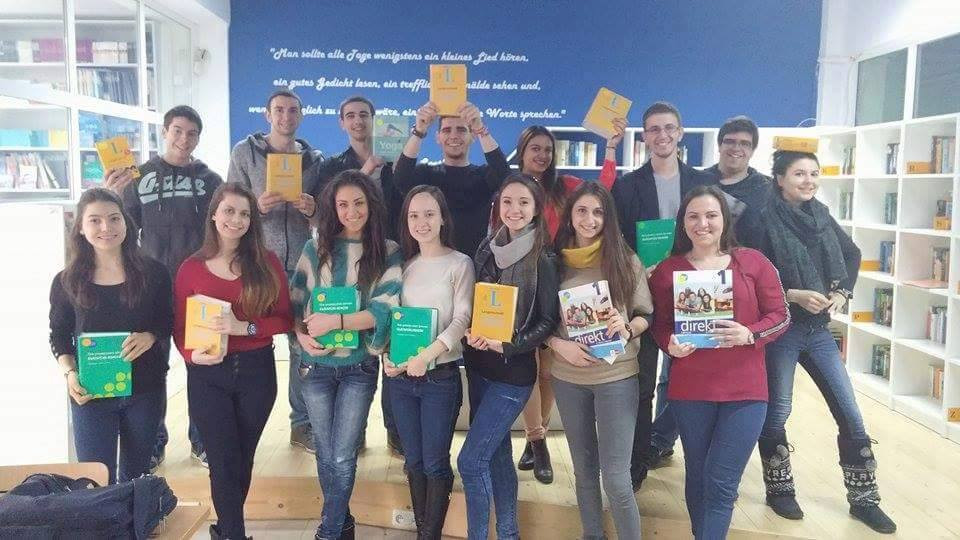
\includegraphics[width=4.5in]{./DSD/dsd.jpg},] 
\end{window}
Помагахме си, давахме си идеи. Кафето се превръщаше в неделима част от 
денонощието ни. И все пак не се чувствахме готови. Дойде писмения. Знаехме, че 
ще е трудно, но знаехме, че трудът на всеки ще се отплати. Бях уплашена. Дали 
подготовката беше достатъчна? Когато прекрачих прага на изпитната зала, осъзнах, 
че това беше решаващият момент. И се почувствах готова. И това мина. 

Дъждовна петъчна сутрин – денят на устния изпит. Предизвикателство беше да бъдеш 
първият изпитан в 9 сутринта.  Колебаех се, \\[7.55cm] страхувах се,  но някакси знаех, че ще 
се справя. Знаех, че всеки от нас ще се справи, защото това бяхме ние. Помагахме 
си, израснахме заедно, преборихме цели четири години немски. И успяхме. Всеки от 
нас влезе и гордо застана пред комисията, готов да защити онова, което трябва. 
Всеки отстояваше мнението си, всеки можеше да го направи. И всеки един от нас 
успя. Дали с C1, или с B2 – всеки от нас достигна своя връх. И после... Свърши. 
Всичко мина. Няколко месеца по-късно сълзи от радост се търкаляха по лицата ни. 
И осъзнахме, че сме далеч от зрелостта.
Последният учебен срок привършва. Справихме се. Успяхме да преминем и през тази 
трудност. Някои по-добре, а други не чак толкова. Но го направихме заедно. И 
заедно осъзнахме, че не сме нищо повече от деца, които гонят мечтите си. Че да 
бъдеш зрял, значи да създаваш мечта, да работиш за нея, да я осъществиш. Може би 
се доближаваме до света на 
големите. С първия голям успех. Ще има още много. Но сега... Сега ще се 
порадваме на първата голяма победа. С любезното съдействие на Немска езикова 
гимназия „Гьоте“ град Бургас.
\end{multicols}


